\documentclass[aspectratio=169]{beamer}
\usetheme{Madrid}
\usecolortheme{beaver}
\usepackage[utf8]{inputenc}
\usepackage[T1]{fontenc}
\usepackage{tikz}
\usepackage{amssymb}
\usepackage{graphicx}
\setbeamertemplate{navigation symbols}{}
\setbeamercolor{title}{fg=white,bg=cyan!60!black}
\setbeamercolor{frametitle}{fg=white,bg=cyan!50!black}
\setbeamercolor{block title}{bg=cyan!15,fg=black}
\setbeamercolor{block body}{bg=cyan!5,fg=black}

\title{Story Studio 3 — Make It Click}
\subtitle{Lesson 1: Click to Reveal}
\author{ByteForge --- Grade 7 --- Game Maker}
\date{}

\begin{document}

\begin{frame}
    \titlepage
\end{frame}

\begin{frame}{onclick — code that waits for a click}
    \Large
    Every block before this ran the instant you pressed Run. "When button is clicked" waits, doing nothing, until a real click happens.

    \begin{center}
    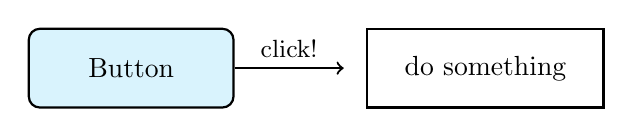
\begin{tikzpicture}[scale=0.9]

        \node[draw, thick, rounded corners, minimum width=2.6cm, minimum height=1cm, fill=cyan!15] (btn) at (0,0) {Button};
        \draw[->, thick] (btn) -- (3,0) node[midway, above] {\small click!};
        \node[draw, thick, minimum width=3cm, minimum height=1cm] (act) at (5,0) {do something};
    \end{tikzpicture}
    \end{center}
\end{frame}

\begin{frame}{onclick — code that waits for a click --- Worked Example}
    \Large
    Worked example: nothing inside "when button is clicked" runs when you press Run — it only runs the moment a real click happens, which is why the checker fires one simulated click to test it.
\end{frame}

\begin{frame}{Your Turn}
    \Large
    Open the student map, find \textbf{Story Studio 3 — Make It Click}, and complete
    the \textbf{Click to Reveal} challenge --- everything you just saw, they now do themselves.
\end{frame}

\end{document}
